\begin{frame}{Directional Stimulus Prompting}
  \begin{itemize}
    \item Prompting technique to better guide the LLM in generating the desired summary.
    \item A tuneable policy LM is trained to generate the hints that guide a black-box frozen LLM.
  \end{itemize}
  \vspace{0.6em}
  \begin{center}
    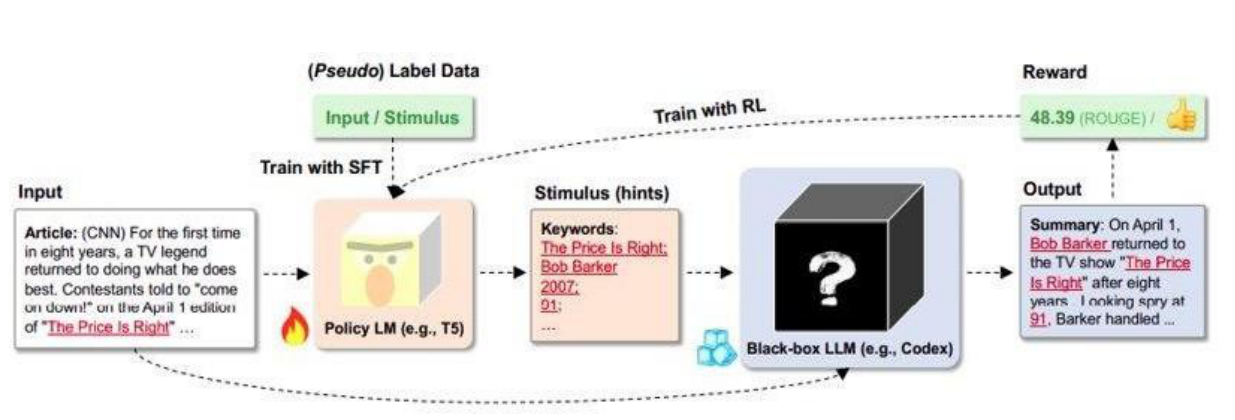
\includegraphics[width=0.8\textwidth,height=0.52\textheight,keepaspectratio]{images/prompting-rag/prompting_directional_stimulus_training.png}
  \end{center}
  \vspace{0.2em}
  {\scriptsize
    \color{gray!75!black}
    Source: Li et al., ``Guiding Large Language Models via Directional Stimulus Prompting'', NeurIPS 2023, \url{https://arxiv.org/abs/2302.11520}
  }
\end{frame}

\begin{frame}{Directional Stimulus Prompting Example}
  \centering
  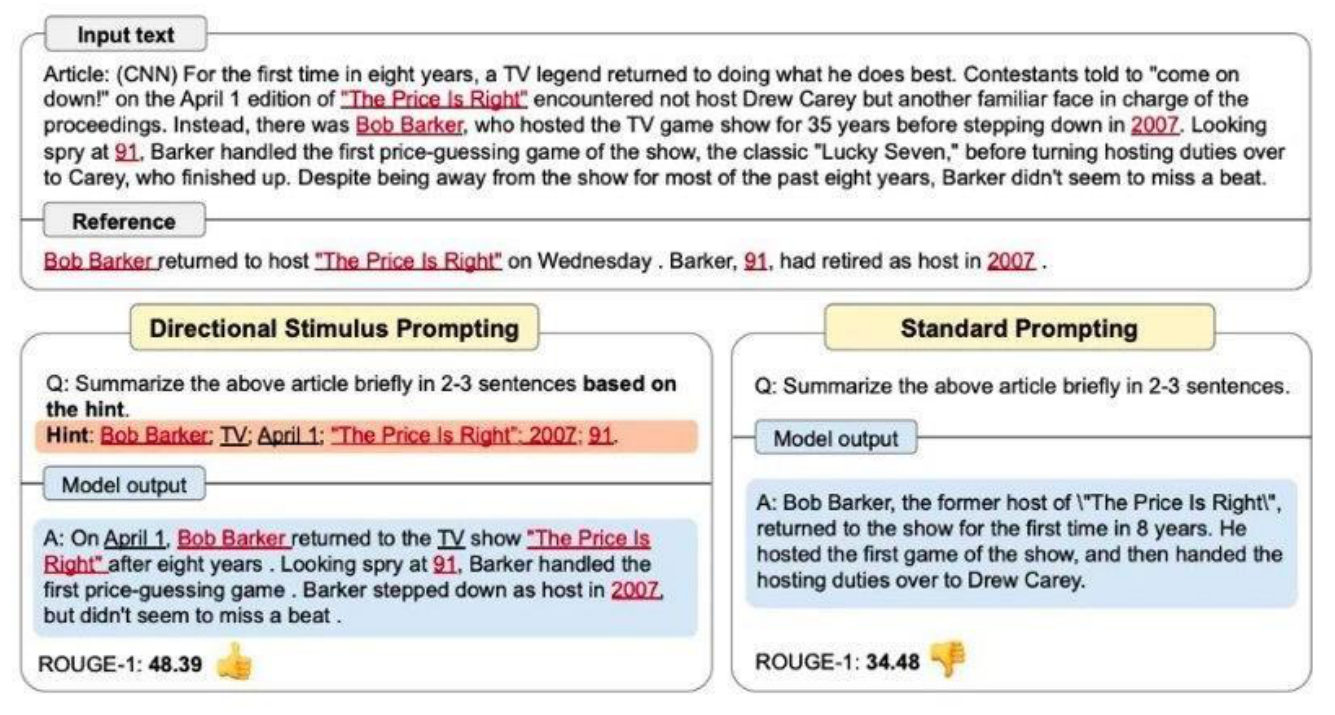
\includegraphics[width=0.9\textwidth, height=0.82\textheight, keepaspectratio]{images/prompting-rag/prompting_directional_stimulus_comparison.png}

  {\scriptsize
    \color{gray!75!black}
    Source: Li et al., NeurIPS 2023, \url{https://arxiv.org/abs/2302.11520}
  }
\end{frame}
